\documentclass{book}
\usepackage[utf8]{inputenc}
\usepackage{graphicx}
\title{Probabilistic Graphical Models}
\author{Huynh Xuan Phung - Coursera}
\date{ }
\usepackage{color}   %May be necessary if you want to color links
\usepackage{hyperref}
\hypersetup{
    colorlinks=true, %set true if you want colored links
    linktoc=all,     %set to all if you want both sections and subsections linked
    linkcolor=blue,  %choose some color if you want links to stand out
} 
\begin{document}
 
\maketitle
 
\tableofcontents

\chapter{Representation}

\section{Introduction}
Model 

\begin{figure}[h]
\centering
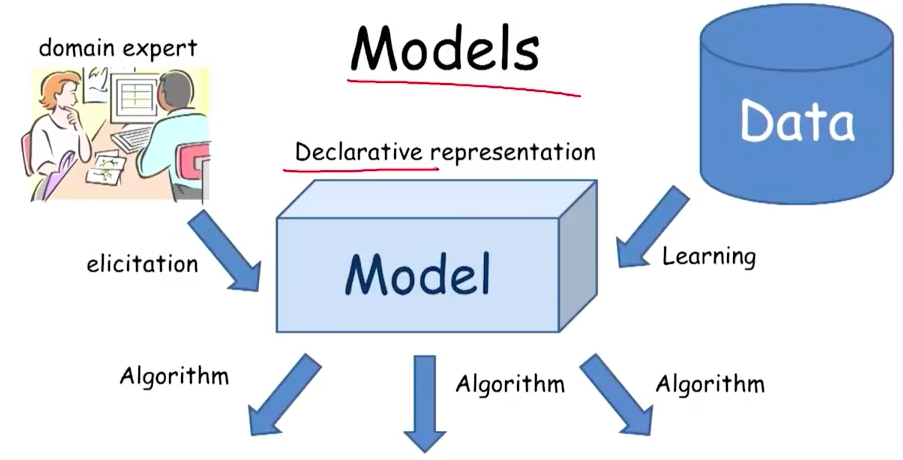
\includegraphics[width=0.7\linewidth]{figures/Models}
\caption{Model is a declarative representation of our understanding of the world}
\label{fig:models}
\end{figure}

It is important because the same representation, that same model can be used in the the context of one algorithms that might answer different kind of questions. Or the same question in more efficient way.

We can construct methodologies the elicit these models from a human extrict, or learn from data or combination.

Uncertainty

--- Partial knowledges of state of the world

--- Noisy observations

--- Phenomena not covered by our model

--- Inherent stochasticity

Probability Theory

--- Declarative representation with clear semantics

--- Powerful reasoning patterns: conditioning decision making

--- Established learning methods

Complex Systems

Graphical Models: Bayesian Networks, Markov Networks (directed or undirected graphs)

Graphical Representation

--- Intuitive and compact data structure

--- Efficient reasoning using general purpose algorithms

--- Sparse parameterization

------ feasible elicitation : by hand

------ learning from data automatically

\subsection{Distribution}
Joint Distribution: P(I,D,G)

Conditioning: observation 1 value of variable ---$>$ Reduction ---$>$ Renormalization $P(I,D,g^1)$  ---$>$ $P(I,D|g^1)$


Marginalization: $\sum_{I}P(I,D) = P(D)$ . Example: you have thrown two 6-sided dice, $D_1$ and $D_2$. $P(D_1,D_2)$ is a joint probability distribution. The probability that $D_2=1$ is equals to $\sum_{i=1}^{6}P(D_1 = i, D_2=1)$.

\subsection{Factors}
A factor is a function or table $\phi(X_1,...,X_k)$

$\phi: Val(X_1,...,X_k) \rightarrow R$

Scope = ${X_1,...,X_k}$

Joint distribution is a factor

Unnormalized measure is a factor

Conditional Probability Distribution (CPD) is a factor P(G|I,D): G in columns while I,D in rows.

Why factors?

--- Fundamental building block for defining distributions in high-dimensional spaces

--- Set of basic operations for manipulating these probability distributions

\section{Bayesian Network (Directed Models)}
\subsection{Semantics and Factorization}
What does random variable depend on?

Draw nodes, edges, each node with a factor is CPD (conditional probability distribution)

A bayesian network is:

--- A directed acyclic graph (DAG) G whose nodes represent the random variables

--- For each node $X_i$ a CPD $P(X_i|Par_G(X_i))$

The BN represent a joint distribution via the chain rule for Bayesian Networks

$P(X_1,...,X_n) = \prod_{i} P(X_i|Par_G(X_i))$

BN is a Legal distribution : $\sum P=1$ and $P>0$

\subsection{Reasoning Pattern}
Causal Reasoning: reasoning going down

Evidential Reasoning: reasoning going up

Inter-causal Reasoning: The probability of class is hard, if we observe the "C" grade and change the posterior probability of high intelligence is goes up

\subsection{Flow of Probabilistic Influence}
When can X influence Y?

X $\rightarrow$ Y

X $\leftarrow$ Y

Active Trails: 

A trail $X_1$ -- ... -- $X_k$ is active if: it has no v-structures $X_{i-1} \rightarrow X_i \leftarrow X_{i+1}$

When can X influence Y given evidence about Z?

A trail $X_1$ --- ... --- $X_k$ is active given Z if:

--- for any v-structure $X_{i-1} \rightarrow X_i \leftarrow X_{i+1} $ we have that $X_i$ or one of its descendants $\in$ Z

--- no other $X_i$ is in Z

Assignment

1. How many parameter to present a CPD. If X have m possibilities the P(X) needs m-1 independent parameters

IF Y have k possibilities, Z have l possibilities then P(X|Y,Z) has (m-1)*k*l independent parameters.

2. Inter-causal reasoning

\begin{figure}[h]
\centering
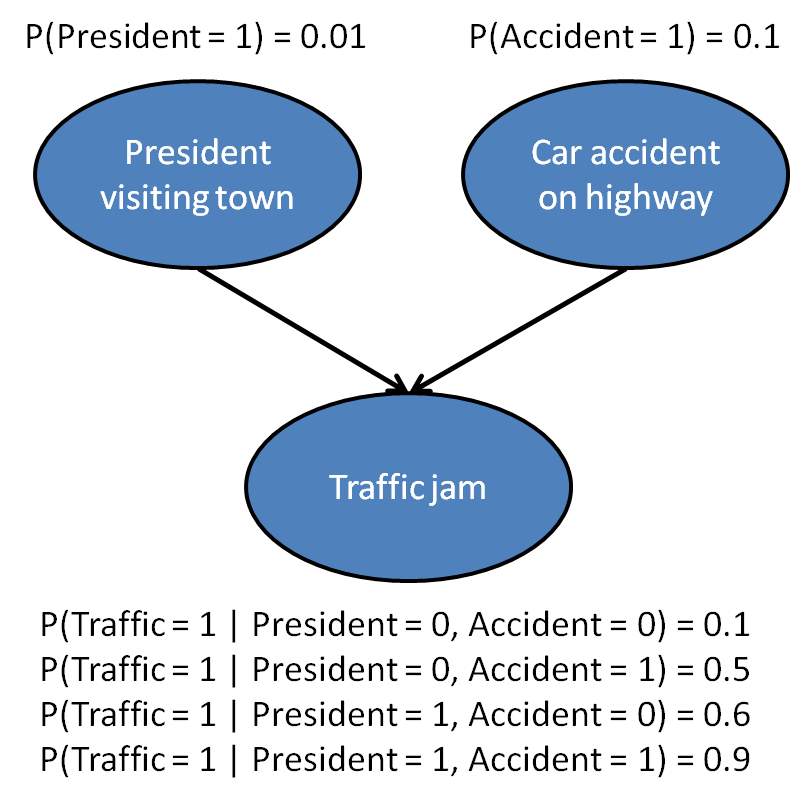
\includegraphics[width=0.7\linewidth]{figures/bayesian_ex1}
\caption{}
\label{fig:bayesianex1}
\end{figure}

To calculate the required values, we can apply Bayes' rule. For instance,

$\frac{P(A=1|T=1,P=1)=P(A=1,T=1,P=1)}{P(T=1,P=1)}$

$=\frac{P(A=1,T=1,P=1)}{(P(A=0,T=1,P=1)+P(A=1,T=1,P=1))}$.

We can then use the chain rule of Bayesian networks to substitute the correct values in, e.g.,

$P(A=1,T=1,P=1)=P(P=1)*P(A=1)*P(T=1|P=1,A=1)$

This example of inter-causal reasoning meshes well with common sense: if we see a traffic jam, the probability that there was a car accident is relatively high. However, if we also see that the president is visiting town, we can reason that the president's visit is the cause of the traffic jam; the probability that there was a car accident therefore drops correspondingly.






 
\end{document}